% !TeX encoding = UTF-8
% !TeX spellcheck = pl_PL

% $Id:$

%Author: Wojciech Domski
%Szablon do ząłożeń projektowych, raportu i dokumentacji z sterowników robotów
%Wersja v.1.0.0
%


%% Konfiguracja:
\newcommand{\kurs}{Sterowniki robot\'{o}w}
\newcommand{\formakursu}{Projekt}

%odkomentuj właściwy typ projektu
\newcommand{\doctype}{Za\l{}o\.{z}enia projektowe}
%\newcommand{\doctype}{Raport}
%\newcommand{\doctype}{Dokumentacja}

%wpisz nazwę projektu
\newcommand{\projectname}{Miecz \'{S}wietlny}

%wpisz akronim projektu
\newcommand{\acronim}{Mi\'{S}}

%zmaiast X wpisz numer grupy projektowej
\newcommand{\nrgrupy}{4}
%wpisz Imię i nazwisko oraz numer albumu
\newcommand{\osobaA}{Patryk \textsc{Knapik}, 226302}
%w przypadku projektu jednoosobowego usuń zawartość nowej komendy
\newcommand{\osobaB}{Wojciech \textsc{Kosicki}, 234506}

%wpisz termin w formie, jak poniżej dzień, parzystość, godzina
\newcommand{\termin}{wtTP11}

%wpisz imię i nazwisko prowadzącego
\newcommand{\prowadzacy}{mgr in\.{z}. Wojciech \textsc{Domski}}

\documentclass[10pt, a4paper]{article}
% W nawiasie klamrowym podana jest klasa dokumentu. Standardowe klasy artykułu
% to: article, amsart, scrartcl, artikel1, artikel2, artikel3.
% W nawiasie prostokątnym deklarowane są opcje dokumentu. Zamiast 10pt
% można podać 11pt lub 12pt. Dokument w dwóch kolumnach uzyskuje się po
% wpisaniu opcji twocolumn, 

%Preambuła dokumentu

% linki w spisie tresci, bibliografi
\usepackage[bookmarks=true,bookmarksnumbered=false,unicode=true,pdftex=true, colorlinks,filecolor=black,linkcolor=black,urlcolor=black,citecolor=black]{hyperref}

%ustawienie rozmiaru papieru
\usepackage[a4paper, left=2.5cm, right=2.5cm, top=2.5cm, bottom=2.5cm, headsep=1.2cm]{geometry}

%rozmaite ustawienia pozwalające okreslić język

%NALEŻY wybrać jeden z pakietów
%\usepackage{polski} %przydatne podczas składania dokumentów w j. polskim
\usepackage[polish]{babel}  % pakiet lokalizujący dokument w języku polskim
%\usepackage[british]{babel}

\usepackage{indentfirst}	% polski styl pisania (np. rozpoczecie pierwszego akapitu
% pod nazwa rozdzialu od wciecia)
%\usepackage[OT4]{fontenc}
\usepackage[utf8]{inputenc} % w miejsce utf8 można wpisać latin2 bądź cp1250,
% w zależności od tego w jaki sposób kodowane są 
% polskie znaki diakrytyczne przy wprowadzaniu 
% z klawiatury.
%kodowanie znaków, zależne od systemu
\usepackage[T1]{fontenc} %poprawne składanie polskich czcionek

%OPEROWANIE NA OBRAZACH
\usepackage{graphicx}       % pakiet graficzny, umożliwiający m.in.
% import grafik w formacie eps
%\usepackage{epstopdf}		% pozwala na importowanie grafik w formacie eps
% przy użyciu pdflatex
\usepackage[update,prepend]{epstopdf}
\usepackage{rotating}       % pakiet umożliwiający obracanie rysunków
\usepackage{subfigure}      % pakiet umożliwiający tworzenie podrysunków
\usepackage{epic}           % pakiet umożliwiający rysowanie w środowisku latex
\usepackage{psfrag}         % pakiet umożliwiający podmianę łańcuchów znaków 
% w plikach eps
%\usepackage{curves}         % pakiet do wykreslania krzywych

%pakiety dodające dużo dodatkowych poleceń matematycznych
\usepackage{amsfonts}       % pakiet z rozmaitymi czcionkami matematycznymi
%\usepackage{amssymb}        % pakiet z rozmaitymi symbolami matematycznymi
\usepackage{amsmath}        % pakiet z rozmaitymi środowiskami matematycznymi

\usepackage{fp}             % pakiet z funkcjami operujacymi 
% na liczbach zmiennoprzecinkowych
\usepackage{calc}           % pakiet umożliwiający operacje arytmetyczne
% na tzw. licznikach (liczbach całkowitych)
\usepackage{leftidx}		% indeksy górne i dolne po lewej stronie

%definicje matematyczne
\providecommand{\abs}[1]{\lvert#1\rvert}
\providecommand{\norm}[1]{\lVert#1\rVert}

%pakiety wspomagające i poprawiające składanie tabel
\usepackage{supertabular}
\usepackage{array}
\usepackage{tabularx}
\usepackage{hhline}
\usepackage{longtable}		% wsparcie dla dlugich tabel
\usepackage{multicol}		% podzial strony na wiele kolumn

%pakiet do BibTex
\usepackage{cite}

\usepackage{url} %pakiet pozawalający na dodawanie adresów url w bibliografi

%pakiet wypisujący na marginesie etykiety równań i rysunków zdefiniowanych przez \label{}, chcąc wygenerować finalną wersję dokumentu wystarczy usunąć poniższą linię
%\usepackage{showlabels}

\usepackage{float}			% lepsza obsluga mechanizmow obiektow plywajacych
% wymuszenie wstawienia np. tabeli, obrazka w danym miejscu przez [H]

\usepackage{listings}       % pakiet dedykowany zrodlom programow
\usepackage{color}


\definecolor{dkgreen}{rgb}{0,0.6,0}
\definecolor{gray}{rgb}{0.5,0.5,0.5}
\definecolor{mauve}{rgb}{0.58,0,0.82}

\lstset{ %
	language=Matlab,                % the language of the code
	basicstyle=\scriptsize,           % the size of the fonts that are used for the code
	numbers=left,                   % where to put the line-numbers
	numberstyle=\tiny\color{gray},  % the style that is used for the line-numbers
	stepnumber=1,                   % the step between two line-numbers. If it's 1, each line 
	% will be numbered
	numbersep=5pt,                  % how far the line-numbers are from the code
	backgroundcolor=\color{white},      % choose the background color. You must add \usepackage{color}
	showspaces=false,               % show spaces adding particular underscores
	showstringspaces=false,         % underline spaces within strings
	showtabs=false,                 % show tabs within strings adding particular underscores
	%frame=single,                   % adds a frame around the code
	rulecolor=\color{black},        % if not set, the frame-color may be changed on line-breaks within not-black text (e.g. comments (green here))
	tabsize=2,                      % sets default tabsize to 2 spaces
	captionpos=b,                   % sets the caption-position to bottom
	breaklines=true,                % sets automatic line breaking
	breakatwhitespace=false,        % sets if automatic breaks should only happen at whitespace
	%title=\lstname,                   % show the filename of files included with \lstinputlisting;
	% also try caption instead of title
	keywordstyle=\color{blue},          % keyword style
	commentstyle=\color{dkgreen},       % comment style
	stringstyle=\color{mauve},         % string literal style
	escapeinside={\%*}{*)},            % if you want to add LaTeX within your code
	morekeywords={*,...},              % if you want to add more keywords to the set
	deletekeywords={...}              % if you want to delete keywords from the given language
}

%polish signs in lst code
\lstset{literate=%
	{ą}{{\k{a}}}1
	{ć}{{\'c}}1
	{ę}{{\k{e}}}1
	{ł}{{\l}}1
	{ń}{{\'n}}1
	{ó}{{\'o}}1
	{ś}{{\'s}}1
	{ż}{{\.z}}1
	{ź}{{\'z}}1
	{Ą}{{\k{A}}}1
	{Ć}{{\'C}}1
	{Ę}{{\k{E}}}1
	{Ł}{{\L}}1
	{Ń}{{\'N}}1
	{Ó}{{\'O}}1
	{Ś}{{\'S}}1
	{Ż}{{\.Z}}1
	{Ź}{{\'Z}}1
}

\usepackage{verbatim}       % pakiet dedykowany rozmaitym wydrukom tekstowym
\usepackage{ifthen}         % pakiet umożliwiający tworzenie prostych programów
% (m.in. zawiera instrukcje powtórzeniowe 
% i warunkowe)
\usepackage{upquote}		%normal quotations marks ' and `

% deklaracje wymagane przez pakiet theorem automatycznie ladowany w przypadku
% klasy dokumentu article
%
\newtheorem{Dn}{Definicja}[section]     % deklaracja srodowiska definicja
\newtheorem{La}[Dn]{Lemat}                % deklaracja srodowiska lemat
\newtheorem{Tm}[Dn]{Twierdzenie}          % deklaracja srodowiska twierdzenie
\newtheorem{Rk}[Dn]{Spostrze{\.z}enie}  % deklaracja srodowiska spostrzezenie
\newtheorem{Am}[Dn]{Algorytm}           % deklaracja srodowiska algorytm
\newtheorem{As}[Dn]{Za{\l}o{\.z}enie}   % deklaracja srodowiska zalozenie
\newtheorem{Pn}[Dn]{Propozycja}           % deklaracja srodowiska propozycja
\newtheorem{Py}[Dn]{W{\l}asno{\'s}{\'c}}  % deklaracja srodowiska wlasnosc
\newtheorem{Cy}[Dn]{Wniosek}              % deklaracja srodowiska wniosek
\newtheorem{Ee}[Dn]{Przyk{\l}ad}        % deklaracja srodowiska przyklad
\newtheorem{Ex}{{\'C}wiczenie}          % deklaracja srodowiska cwiczenie

%helps to specify width of a column in table
%\begin{tabular}{|C{1cm}|c|c|c|c|c|c|c|c|c|c|}
%first column will have widht of 1cm
\newcolumntype{L}[1]{>{\raggedright\let\newline\\\arraybackslash\hspace{0pt}}m{#1}}
\newcolumntype{C}[1]{>{\centering\let\newline\\\arraybackslash\hspace{0pt}}m{#1}}
\newcolumntype{R}[1]{>{\raggedleft\let\newline\\\arraybackslash\hspace{0pt}}m{#1}}

\sloppy			%zawija bardzo długie linie

%\pagenumbering{gobble}% Remove page numbers (and reset to 1)

	
\begin{document}

\def\tablename{Tabela}	%zmienienie nazwy tabel z Tablica na Tabela

\begin{titlepage}
	\begin{center}
		\textsc{\LARGE \formakursu}\\[1cm]		
		\textsc{\Large \kurs}\\[0.5cm]		
		\rule{\textwidth}{0.08cm}\\[0.4cm]
		{\huge \bfseries \doctype}\\[1cm]
		{\huge \bfseries \projectname}\\[0.5cm]
		{\huge \bfseries \acronim}\\[0.4cm]
		\rule{\textwidth}{0.08cm}\\[1cm]
		
		\begin{flushright} \large
		\emph{Skład grupy (\nrgrupy):}\\
		\osobaA\\
		\osobaB\\[0.4cm]
		
		\emph{Termin: }\termin\\[0.4cm]

		\emph{Prowadzący:} \\
		\prowadzacy \\
		
		\end{flushright}
		
		\vfill
		
		{\large \today}
	\end{center}	
\end{titlepage}

\newpage
\tableofcontents
\newpage

\section{Opis projektu}
\label{sec:OpisProjektu}
Projekt zakłada stworzenie urządzenia które będzie wykorzystywało dane z akcelerometru do generowania dźwięków o odpowiedniej częstotliwości za pomocą układu DAC. Dźwięki będą generowane w taki sposób, żeby imitowały pracę poruszanego miecza świetlnego znanego chociażby z filmów pt. \textit{Star Wars}. 

\section{Założenia projektowe} %jak będzie buczeć inaczej w idlu i inaczej podczas ruszania to już będę zadowolony
	\begin{flushleft}
	Założenia podstawowe funkcjonalności:\\
	\end{flushleft}
	\begin{itemize}
		\item Dioda LED RGB imitująca ostrze miecza.
		\item Wybór koloru diody przez użytkownika za pomocą przycisku z palety kolorów w jakich najczęściej występują miecze świetlne.
		\item Miecz ma generować dźwięk, przypominający ten znany z miecza świetlnego, za pomocą DACa - ruch mieczem ma zmieniać ton i częstotliwość dzwięku w podobny sposób jak robi to miecz świetlny.
		\item Możliwość włączania i wyłączania miecza za pomocą przycisku.
		\item Miecz wyłączony nie generuje dźwięków, a także wyłącza LED RGB.
	\end{itemize}
	\vspace{5mm}
	\begin{flushleft}
	Założenia dodatkowe funkcjonalności (wdrażane po tym jak założenia podstawowe funkcjonalności zostaną spełnione):\\
	\end{flushleft}
	\begin{itemize}
		\item Możliwość wyboru koloru z palety True color (24-bit).
		\item Dźwięk włączania i wyłączania miecza odtwarzany z zewnętrznej pamięci flash komunikującej się z mikrokontrolerem za pomocą QSPI.
		\item Szkielet na baterię (np. power bank USB), głośnik oraz pasek LED RGB.
	\end{itemize}
	\vspace{5mm}
	\begin{flushleft}
	Założenia budowy programu:\\
	\end{flushleft}
	\begin{itemize}
		\item Implementacja bazująca na przerwaniach - główna pętla obsługuje zdarzenia po ustawieniu flagi w przerwaniu.
		\item Wykorzystanie programu \textit{CubeMX} dostarczanego przez firmę \textit{ST} w celu wygenerowania kodu potrzebnego do w/w peryferiów.
	\end{itemize}

	

\section{Harmonogram pracy} %tutaj powinny być chyba kamienie milowe i wykres Gantta, DODAC TERMINY!!
	\begin{flushleft}
	Kamienie milowe zostały pogrubione i podkreślone\\
	\end{flushleft}
	\begin{enumerate}
		\item Wygenerowanie projektu bazowego w CubeMX.\\
		\underline {Termin: 06.03 - 08.03}
		\item Implementacja obsługi DACa.\\
		\underline {Termin: 09.03 - 22.03}
		\item Implementacja obsługi akcelerometru.\\
		\underline {Termin: 09.03 - 22.03}
		\item Opracowanie algorytmu generującego dźwięk zbliżony do dźwięku miecza świetlnego.\\
		\underline {Termin: 15.03 - 29.03}
		\item Obsługa diody LED RGB imitującej ostrze za pomocą PWM.\\
		\underline {Termin: 30.03 - 02.04}
		\textbf{\item \underline{Implementacje głównej pętli programu (połączenie akcelerometru z układem DAC).}}\\
		\underline {Termin: 03.04 - 09.04}
		\item Opracowanie wstępnej dokumentacji technicznej po spełnieniu założeń podstawowych.\\
		\underline {Termin: 10.04 - 17.04}
		\item Implementacja obsługi pamięci flash oraz wgrywanie dźwięków za pomocą USB.\\
		\underline {Termin: 18.04 - 02.05}
		\item Implementacja odgrywania dźwięków włączania i wyłączania miecza świetlnego.\\
		\underline {Termin: 03.05 - 10.05}
		\item Implementacja wyboru koloru z palety True color (24-bit) - obsługa przycisków, wyświetlacza i PWM.\\
		\underline {Termin: 18.04 - 25.04}
		\textbf{\item \underline{Rozbudowa głównej pętli programu o obsługę pamięci flash i wyboru koloru z palety.}}\\
		\underline {Termin: 11.05 - 18.05}
		\item Aktualizacja dokumentacji technicznej po spełnieniu założeń dodatkowych.\\
		\underline {Termin: 26.04 - 22.05}
		\item Budowa ramy na komponenty oraz ostrze.\\
		\underline {Termin: 23.05 - 31.05}
	\end{enumerate}
	\begin{figure}[h]
	\centering
	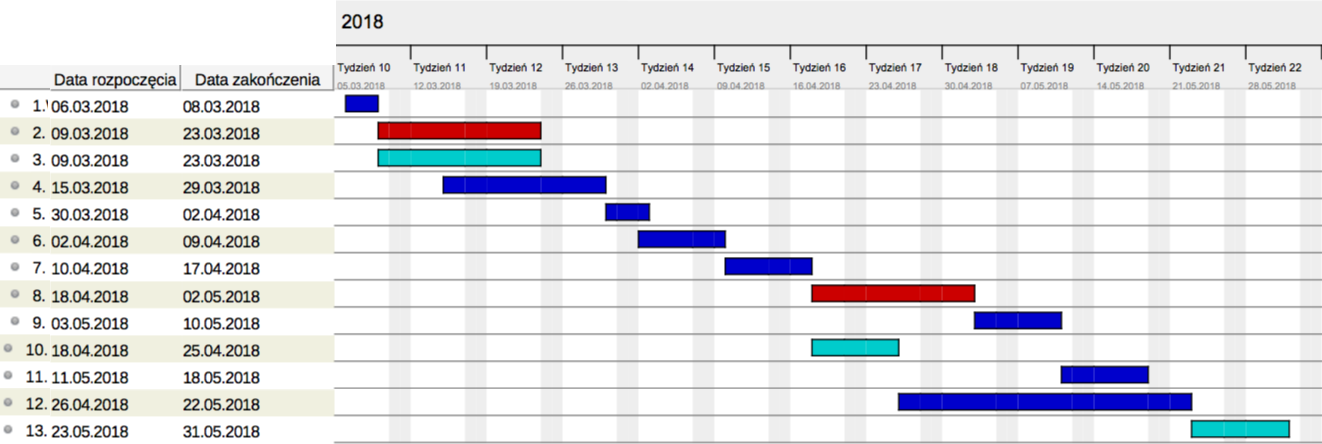
\includegraphics[width=\linewidth]{gantt.png}
	\caption{Wykres Gantta}
	\end{figure}
	
	
	\section{Opis kamieni milowych}
	
	\begin{enumerate}
	
	\item \textbf{Implementacje głównej pętli programu (połączenie akcelerometru z układem DAC).}
	Duża część pracy związana z tym punktem, będzie zawierać się w podstawowej implementacji przyrządów zewnętrznych. Gdy etap implementacji obsługi akcelerometru i DACa zostanie zakończony, to kolejnym krokiem będzie implementacja podstawowej pętli, na bazie której układ będzie generował dźwięk w zależności od ruchu.
	
	\item \textbf{Rozbudowa głównej pętli programu o obsługę pamięci flash i wyboru koloru z palety.}
	Pierwszy kamień milowy jest podstawą do działania całego projektu. W rozszerzonej wersji planowane jest odtwarzanie dźwięków których generowanie za pomocą mikrokontrolera jest bardzo trudne, mianowicie dźwięki otwierania, zamykania i uderzenia miecza. Dodatkową funkcjonalnością jest możliwość wyboru dowolnego koloru z palety True color (24-bit) przez użytkownika. Kiedy ten etap zostanie zrealizowany będzie można zbudować prototypową ramę na ostrze oraz urządzenia niezbędne do samowystarczalnego działania miecza.
	
	\end{enumerate}
	
\newpage
\section{Podział pracy} %tutaj też zakres prac 
	
	\begin{itemize}
		\item Patryk Knapik:
			\begin{enumerate}
				\item Implementacja obsługi DAC.
				\item Implementacja obsługi pamięci flash oraz komunikacji USB.
			\end{enumerate}
		\item Wojciech Kosicki:
			\begin{enumerate}
				\item Implementacja obsługi akcelerometru.
				\item Implementacja wyboru koloru z palety True color (24-bit).
				\item Budowa ramy.
			\end{enumerate}
		\item Zadania wspólne:
			\begin{enumerate}
				\item Opracowanie algorytmu generującego dźwięk zbliżony do dźwięku miecza świetlnego.
				\item Implementacja głównej pętli programu.
				\item Opracowanie wstępnej dokumentacji technicznej.
				\item Rozbudowa głównej pętli programu.
				\item Opracowanie finalnej dokumentacji technicznej.
			\end{enumerate}
	\end{itemize}

\section{Podsumowanie}
Temat projektu został dobrany w taki sposób, aby opanować podstawowe umiejętności programowania mikrokontrolerów STM32 jednocześnie tworząc coś ciekawego i zjawiskowego. Na całym świecie miliony fanów szermierki na miecze świetlne walczą ze sobą bronią symulującą wygląd miecza świetlnego. Pomimo takiej popularności i widowiskowości, nie stworzono do tej pory systemu, który by generował charakterystyczny dźwięk tego oręża. Projekt będzie próbą wyjścia na przeciw tym problemom. 

Z uwagi na mnogość peryferiów i małe doświadczenie konstruktorów, projekt ten może być nie małym wyzwaniem.
Niezależnie od komplikacji, plan realizacji zadań projektowych został podzielony pomiędzy dwójkę wykonującą zadanie, w zamyśle był równy podział prac, więc może podlegać on zmianom w taki sposób, żeby to założenie zostało spełnione.
\newpage
\addcontentsline{toc}{section}{Bibilografia}
\bibliography{bibliografia}
\bibliographystyle{plain}


\end{document}







































